\documentclass{article}

\usepackage[utf8]{inputenc}
\usepackage{amsmath}
\usepackage{amsfonts}
\usepackage{amssymb}
\usepackage{graphicx}

\title{\vspace*{-3.5cm}Homework for Linear Algebra \\October 18, 2024} 
\author{Chengyu Zhang}
\date{}

\begin{document}

\maketitle

\paragraph{Exercise 1.}
  \paragraph{1.1}
  \textit{
    From the definition of row echelon form, for the pivot columns $j_1 \cdots j_r$ 
    \[
    1 \leq j_1 < j_2 \cdots < j_r \leq n
    \]
    And the ith pivot must be in the ith row.
    So after the reduce, matrix A must be reduced as the form 
    \[
    \begin{bmatrix}
        \mathbf{U} & \mathbf{X}\\
        \mathbf{0} & \mathbf{0}
    \end{bmatrix}
    \]
    Where $\mathbf{U}$ is a r*r uppper-trangular matrix. So the pivots columns must stays the same.
  }
  \paragraph{1.2}
  \textit{
    For the reduced row echelon form, since the value of pivots is 1. We can perform row mulitplications to arbitary row echelon form matrices.\\
    From previous proof, we know that the position won't change. When we unify the value, the reduced row echelon form will be unique.
  }

\paragraph{Exercise 2.}
  \paragraph{2.1}
  \textit{
     Start from r=0. Each time we choose a vector $\mathbf{v} \in V$
     \[
     \mathbf{v} \in V \setminus span(\{\mathbf{v}_{i_1}\cdots \mathbf{v}_{i_r}\})
     \]
     And add it to the $\mathbf{v}_{i_r}$ subset.\\
     Repeat the process until we cannot find any $\mathbf{v}$.Since $ r \leq n$ the process must will have a end.\\
     Now we have \[
        V \subseteq span(\{\mathbf{v}_{i_1}\cdots \mathbf{v}_{i_r}\}) \Rightarrow  span(\{\mathbf{v}_{i_1}\cdots \mathbf{v}_{i_r}\}) =span(\{\mathbf{v}_{1}\cdots \mathbf{v}_{n}\})
     \]
     and each pair of vectors in the subset are linearly independent.
     From definition, it is a basis for $span(\{\mathbf{v}_{1}\cdots \mathbf{v}_{n}\})$
  }

  \paragraph{2.2}
  \textit{
    $\Rightarrow$ From $\textbf{2.1}$, there exists r vectors that consist the basis of  \[
    span( \{ \mathbf{v}_1 \cdots \mathbf{v}_n\})
    \]
    Assume $\mathbf{v}_1 \cdots \mathbf{v}_n$ are not linearly independent. Now
    \[
    r < n \text{ and } dim(span(\{\mathbf{v}_1 \cdots \mathbf{v}_n\})) = dim (span (\{\mathbf{v}_{i_1} \cdots \mathbf{v}_{ir}\})) = r 
    \]
    Contradict!
  } \\
  \textit{
    $\Leftarrow$ From the definition of dimension and basis.\\
    Since $\{\mathbf{v}_1 \cdots \mathbf{v}_n\}$ are linearly independent. It is a basis of $span(\{\mathbf{v}_1 \cdots \mathbf{v}_n\})$
    So the dimension of $span(\{\mathbf{v}_1 \cdots \mathbf{v}_n\})$ is n.
  }
\paragraph{Exercise 3.}
  \textit{
     Assume AB = C. First prove $rank(C) \leq rank(A)$ Assume 
     \[
     C =\begin{bmatrix}
        \mathbf{c}_1 & \cdots & \mathbf{c}_n
     \end{bmatrix} , 
     A = \begin{bmatrix}
        \mathbf{a}_1 & \cdots & \mathbf{a}_n
     \end{bmatrix} 
     \]
     \[
     \mathbf{c_i}= \sum_{j=1}^{n}b_{ji}\mathbf{a}_j
     \]
     Let $\{\mathbf{a}_1, \cots , \mathbf{a}_r\}$ be a basis of C(A).
     \[
     \mathbf{c}_i \text{ can be represented by }\{\mathbf{a}_1, \cots , \mathbf{a}_n\} \Rightarrow \mathbf{c}_i \text{ can be represented by }\{\mathbf{a}_1, \cots , \mathbf{a}_r\}
     \]
     For any $\mathbf{v} \in C(C)$, it can be represented by $\{\mathbf{c}_1, \cots , \mathbf{c}_n\}$.$\Rightarrow$ It can be represented by $\{\mathbf{a}_1, \cots , \mathbf{a}_r\}$
     From previous knowledge
     \[
     dim(C(C))\leq dim(C(A)) \Rightarrow rank(AB) \leq rank(B)
     \]
  } \\
  \textit{
    Next prove $rank(C) \leq rank(B)$ 
    The process is exactly the same as the former one. The only difference is to view the row vectors in AB as linear combinations of row vectors in B.
  }
\paragraph{Exercise 4.}
  \[
  \begin{bmatrix}
    -1 & 3 & 5\\
    -2 & 6 & 10\\
  \end{bmatrix} \Rightarrow
  \begin{bmatrix}
    -1 & 3 & 5\\
    0 & 0 & 0\\
  \end{bmatrix} 
  \]
  \[
  A\mathbf{x}=\mathbf{0} \Rightarrow \begin{bmatrix}
    -1 & 3 & 5\\
    0 & 0 & 0\\
  \end{bmatrix} \begin{bmatrix}
    x_1\\x_2\\x_3
  \end{bmatrix} = \mathbf{0}
  \Rightarrow
  \left\{
  \begin{aligned}
    -x_1+3x_2+5x_3=0\\
    0x_1+0x_2+0x_3=0
  \end{aligned}
  \right.
  \]
  \[
  \mathbf{s}_1=\begin{bmatrix}
    3 \\ 1 \\ 0
  \end{bmatrix}
  \mathbf{s}_2 = \begin{bmatrix}
    5 \\ 0 \\ 1
  \end{bmatrix}
  \]
\[
  \begin{bmatrix}
    -1 & 3 & 5\\
    -2 & 6 & 7\\
  \end{bmatrix} \Rightarrow
  \begin{bmatrix}
    -1 & 3 & 5\\
    0 & 0 & -3\\
  \end{bmatrix} 
  \]
  \[
  A\mathbf{x}=\mathbf{0} \Rightarrow \begin{bmatrix}
    -1 & 3 & 5\\
    0 & 0 & -3\\
  \end{bmatrix} \begin{bmatrix}
    x_1\\x_2\\x_3
  \end{bmatrix} = \mathbf{0}
  \Rightarrow
  \left\{
  \begin{aligned}
    -x_1+3x_2+5x_3=0\\
    0x_1+0x_2-3x_3=0
  \end{aligned}
  \right.
  \]
  \[
  \mathbf{s}_1=\begin{bmatrix}
    3 \\ 1 \\ 0
  \end{bmatrix}
  \]
\paragraph{Exercise 5.}
\begin{figure}[h]
    \centering
    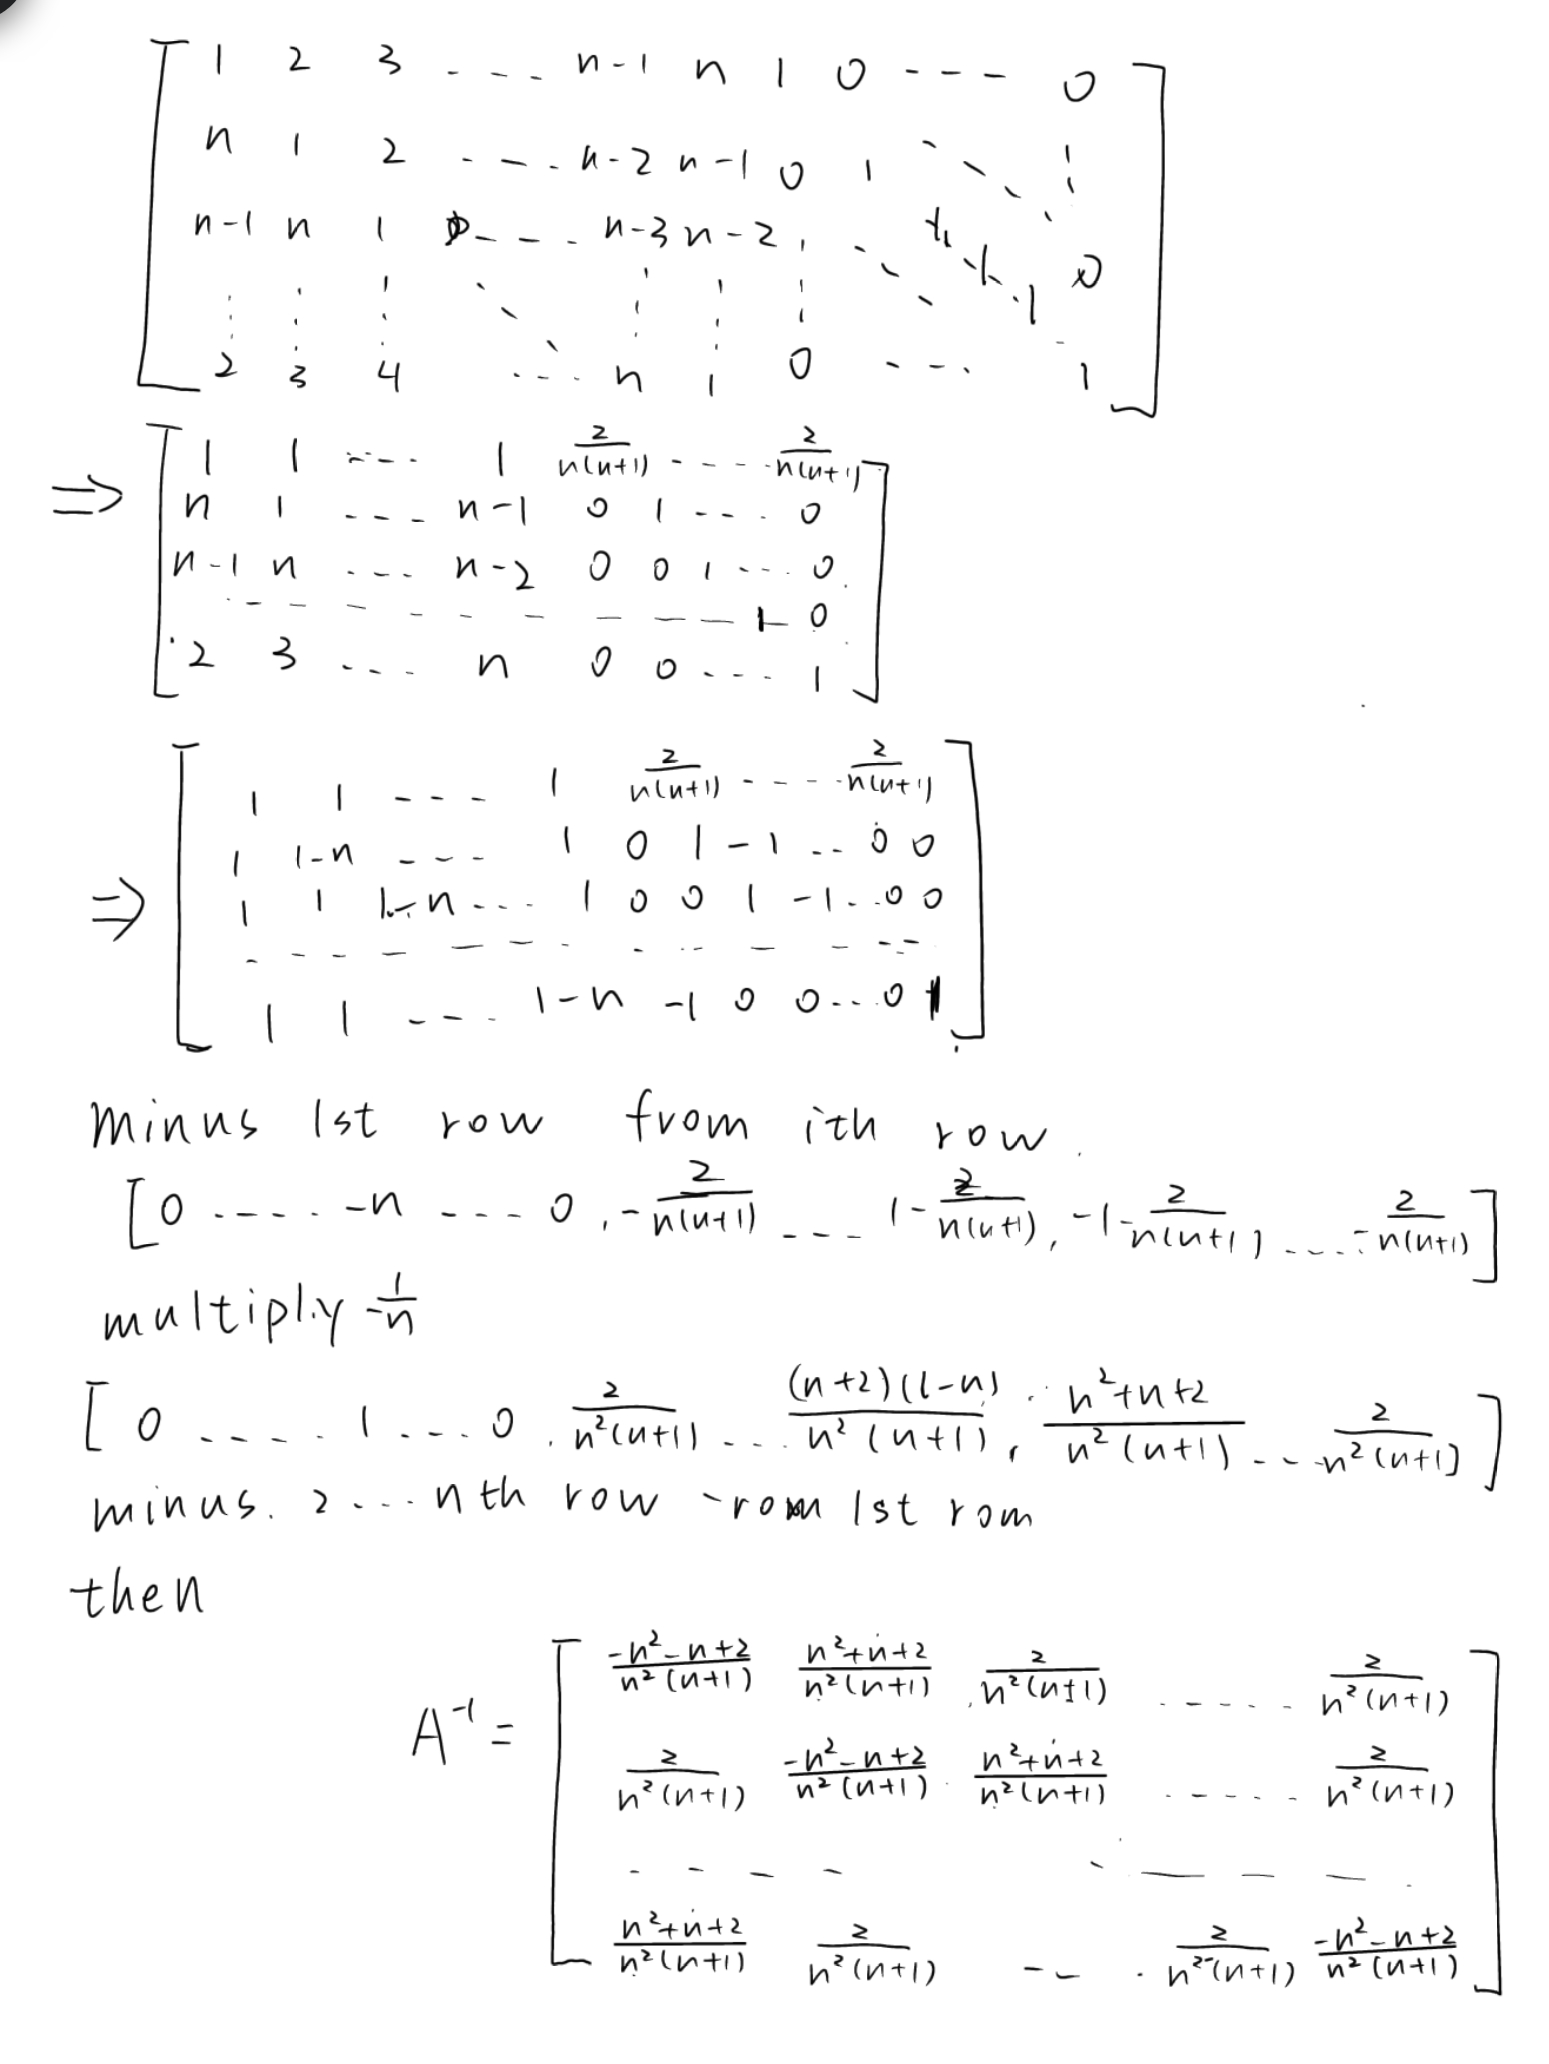
\includegraphics[width=1.0\textwidth]{Capture.jpg}
    \caption{The process}
    \label{fig:example_image}
\end{figure}
\end{document}